Neste capítulo, são apresentados os resultados obtidos através da aplicação da biblioteca desenvolvida aos problemas-exemplo descritos no Capítulo \ref{cap:metodologia}. Para cada problema, são mostrados os gráficos das trajetórias encontradas, bem como a evolução temporal das variáveis de estado e controle. Além disso, são feitas análises comparativas com resultados da literatura, quando disponíveis, e discussões sobre a qualidade das soluções obtidas.

A apresentação dos resultados está organizada na mesma ordem dos problemas-exemplo: inicialmente, são mostrados os resultados do problema de movimento simples em uma dimensão na Seção \ref{subsec:movimento-simples}; em seguida, os resultados do problema da braquistócrona na Seção \ref{subsec:braquistocrona}; e, por fim, os resultados do problema de trajetória do eVTOL na Seção \ref{subsec:evtol}. Para cada problema, são também discutidos aspectos específicos da implementação e eventuais desafios encontrados durante o processo de otimização.

\section{Movimento simples em uma dimensão}
\label{sec:resultados-movimento-simples}

Como parâmetros para a resolução deste problema, utilizou-se $m=1 \, \si{\kilo\gram}$, $s_{x,0}=0 \, \si{\meter}$, $s_{x,f}=1 \, \si{\meter}$, $t_0=0 \, \si{\second}$ e $t_f=1 \, \si{\second}$. Como chute inicial, interpolou-se linearmente os valores iniciais e finais das variáveis de estado e entre os valores $1 \, \si{\newton}$ e $-1 \, \si{\newton}$ para a variável de controle, como mostrado na Figura \ref{fig:resultados-movimento-simples-chute}.

\begin{figure}
    \centering
    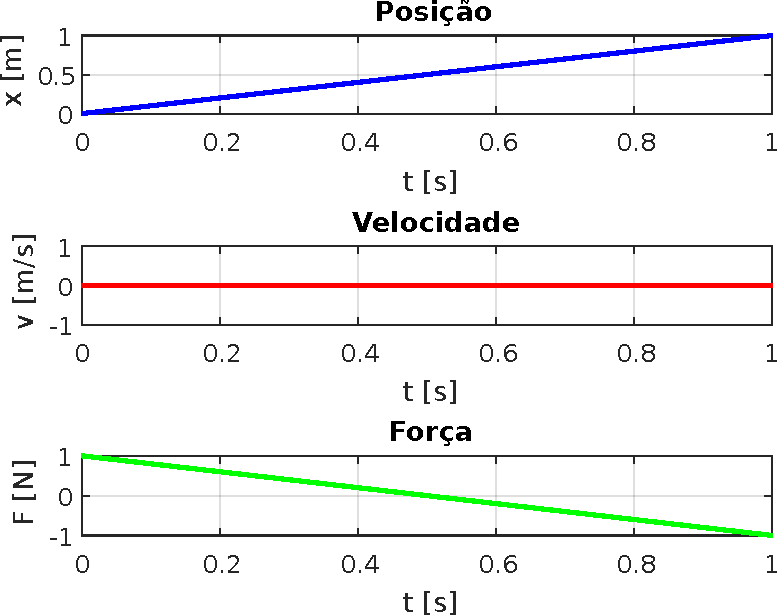
\includegraphics[width=0.65\textwidth]{Cap4/figuras/movimento-simples-chute.pdf}
    \caption{Chute inicial para o problema de movimento simples em uma dimensão.}
    \label{fig:resultados-movimento-simples-chute}
\end{figure}

Como opções do solver, foram utilizados $n=30$ pontos de colocação, sem necessidade de refinamento da malha e nem de ajustes extras de parâmetros para que houvesse convergência para a solução ótima. O resultado é apresentado na Figura \ref{fig:resultados-movimento-simples}.

\begin{figure}[H]
    \centering
    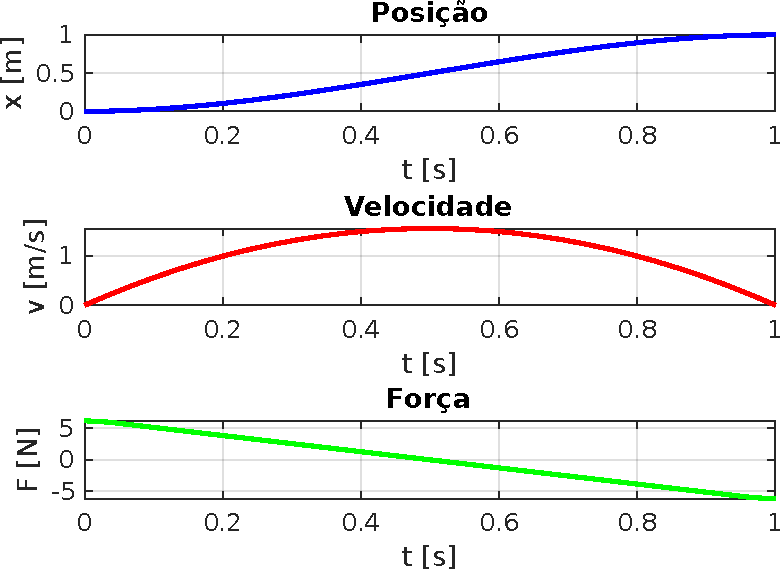
\includegraphics[width=0.65\textwidth]{Cap4/figuras/movimento-simples.pdf}
    \caption{Trajetória ótima do problema de movimento simples em uma dimensão.}
    \label{fig:resultados-movimento-simples}
\end{figure}


\section{Pêndulo invertido}
\label{sec:resultados-pendulo-invertido}

Para a resolução deste problema, utilizou-se $m=1 \, \si{\kilo\gram}$, $l=0,5 \, \si{\meter}$, $b=0,1 \, \si{\newton\second\per\meter}$ e $g=9,81 \, \si{\meter\per\second\squared}$ como parâmetros. Não foi necessário utilizar um chute inicial elaborado, uma vez que o solver encontrou a solução ótima sem dificuldades.

Como opções do solver, utilizou-se uma sequência de refinamento da malha, com $n=[30, 60]$ pontos de colocação. Além disso, apenas aumentou-se o número máximo de avaliações da função por iteração para que o solver convergisse para a solução ótima. O resultado é apresentado na Figura \ref{fig:resultados-pendulo-invertido}.

\begin{figure}[H]
    \centering
    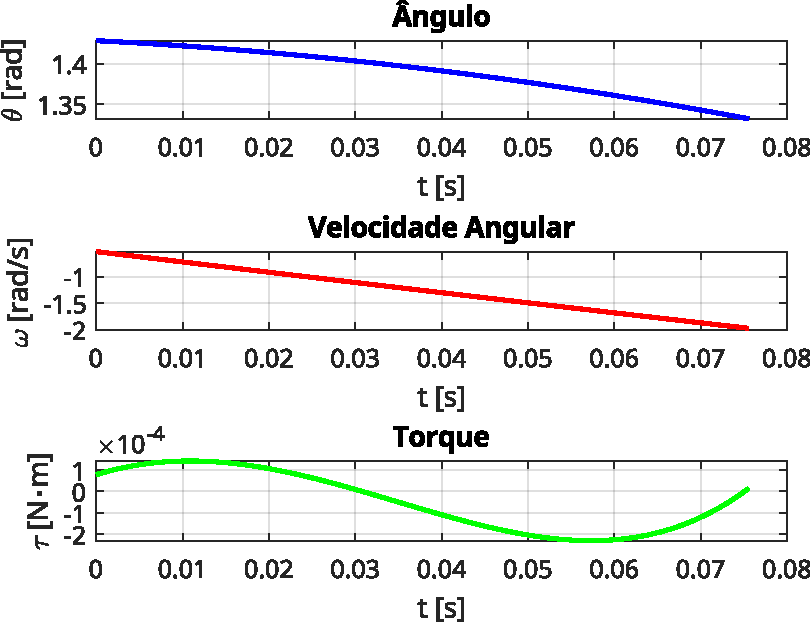
\includegraphics[width=0.65\textwidth]{Cap4/figuras/pendulo-invertido.pdf}
    \caption{Trajetória ótima do problema de pêndulo invertido.}
    \label{fig:resultados-pendulo-invertido}
\end{figure}

\section{Manobra de mudança de faixa}
\label{sec:resultados-manobra-mudanca-faixa}

Como parâmetros para a resolução deste problema, utilizou-se $a_{max}=2 \, \si{\meter\per\second\squared}$, $v_{alvo}=15 \, \si{\meter\per\second}$, $w_{faixa}=3,5 \, \si{\meter}$ e $x_f=75 \, \si{\meter}$ como parâmetros. Também não foi necessário utilizar um chute inicial elaborado, uma vez que o solver encontrou a solução ótima sem dificuldades.

Como opções do solver, utilizou-se uma sequência de refinamento da malha, com $n=[20, 40, 80]$ pontos de colocação. Além disso, assim como no problema do pêndulo invertido, apenas ajustou-se o número máximo de avaliações da função por iteração para que o solver convergisse para a solução ótima. O resultado é apresentado na Figura \ref{fig:resultados-manobra-mudanca-faixa}.

\begin{figure}[H]
    \centering
    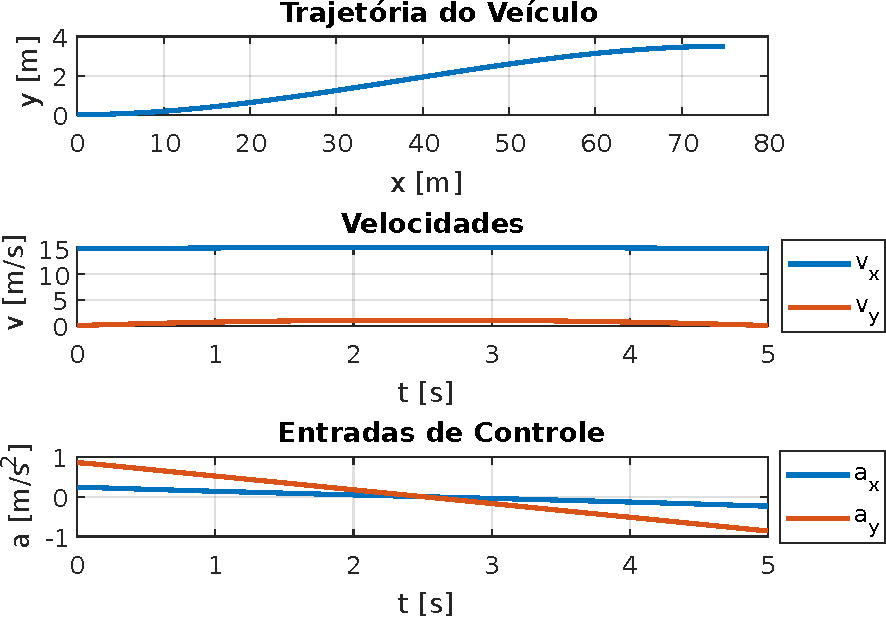
\includegraphics[width=0.77\textwidth]{Cap4/figuras/manobra-mudanca-faixa.pdf}
    \caption{Trajetória ótima do problema de manobra de mudança de faixa.}
    \label{fig:resultados-manobra-mudanca-faixa}
\end{figure}

\section{Braquistócrona}
\label{sec:resultados-braquistocrona}

Para a resolução deste problema, utilizou-se $m=1 \, \si{\kilo\gram}$, $s_{0}=(0,0) \, \si{\meter}$, $s_{f}=(5,-5) \, \si{\meter}$ e $v_0=0 \, \si{\meter\per\second}$ como parâmetros. Como chute inicial, utilizou-se uma parábola horizontal, como mostrado na Figura \ref{fig:resultados-braquistocrona-chute}.

\begin{figure}[H]
    \centering
    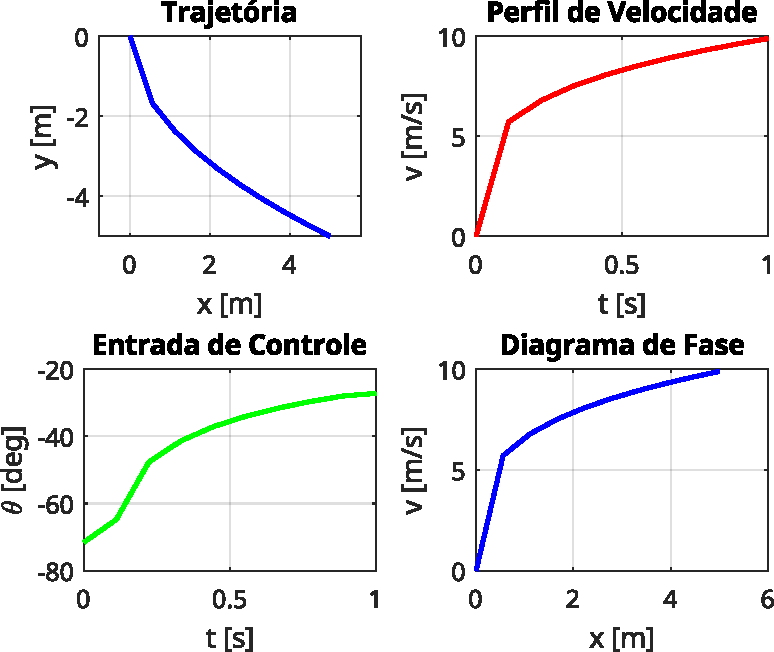
\includegraphics[width=0.68\textwidth]{Cap4/figuras/braquistocrona-chute.pdf}
    \caption{Chute inicial para o problema de braquistócrona.}
    \label{fig:resultados-braquistocrona-chute}
\end{figure}

Como opções do solver, foi utilizada uma sequência de refinamento da malha, com $n=[10, 20, 40]$ pontos de colocação. Além disso, foram utilizadas diversas outras opções de parâmetros para que o solver convergisse para a solução ótima, como o uso de um algoritmo de otimização mais robusto e uma tolerância para a verificação de restrições mais restritiva. Apesar dos esforços, o solver não convergiu para a solução ótima na última iteração, de modo que não se encontrou a solução ótima. Ainda assim, encontrou-se um resultado factível, o qual é apresentado na Figura \ref{fig:resultados-braquistocrona}.

\begin{figure}[H]
    \centering
    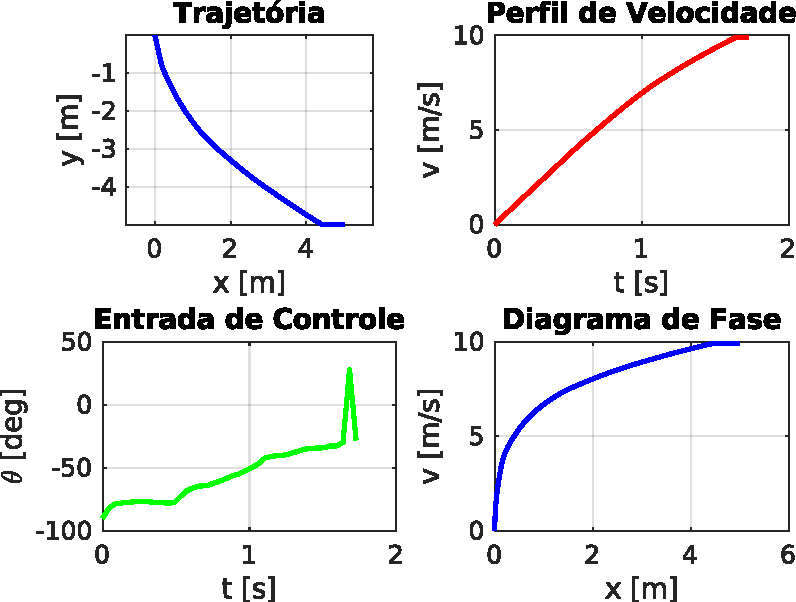
\includegraphics[width=0.7\textwidth]{Cap4/figuras/braquistocrona.pdf}
    \caption{Trajetória ótima do problema de braquistócrona.}
    \label{fig:resultados-braquistocrona}
\end{figure}

Na Figura \ref{fig:resultados-braquistocrona-comparacao} é apresentada a comparação entre a solução obtida e a solução analítica do problema, a qual é uma ciclóide.

\begin{figure}[H]
    \centering
    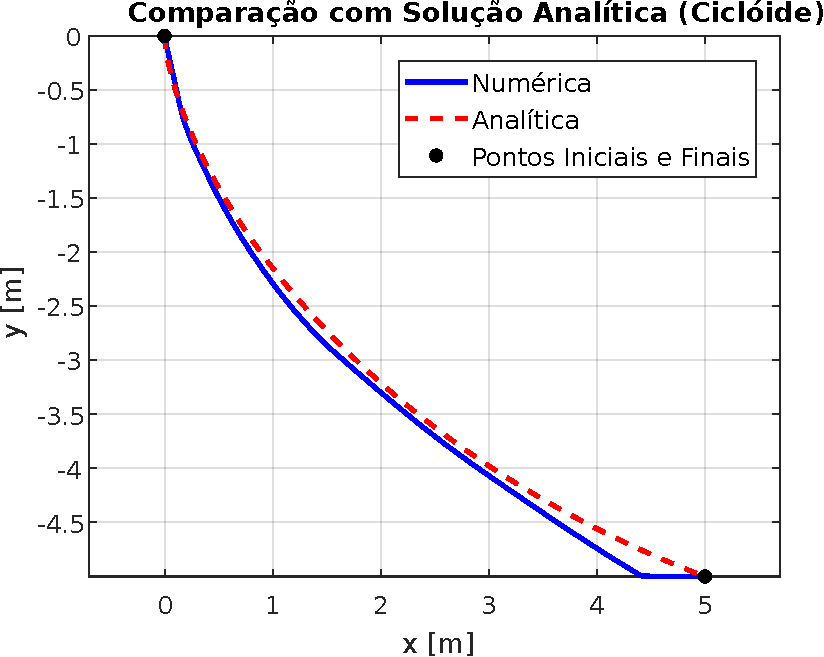
\includegraphics[width=0.65\textwidth]{Cap4/figuras/braquistocrona-comparacao.pdf}
    \caption{Comparação entre a solução obtida e a solução analítica.}
    \label{fig:resultados-braquistocrona-comparacao}
\end{figure}


\section{Trajetória do eVTOL}
\label{sec:resultados-evtol}

O problema considerado é o caso base do trabalho de referência, utilizando-se os mesmos parâmetros nele apresentados. Testou-se também a utilização do mesmo chute inicial, mas sem sucesso. Desse modo, construiu-se um chute inicial fisicamente plausível utilizando-se um polinômio de terceiro grau para a trajetória e respeitando as relações entre as variáveis de estado e controle, como mostrado na Figura \ref{fig:resultados-evtol-chute}.

\begin{figure}[H]
    \centering
    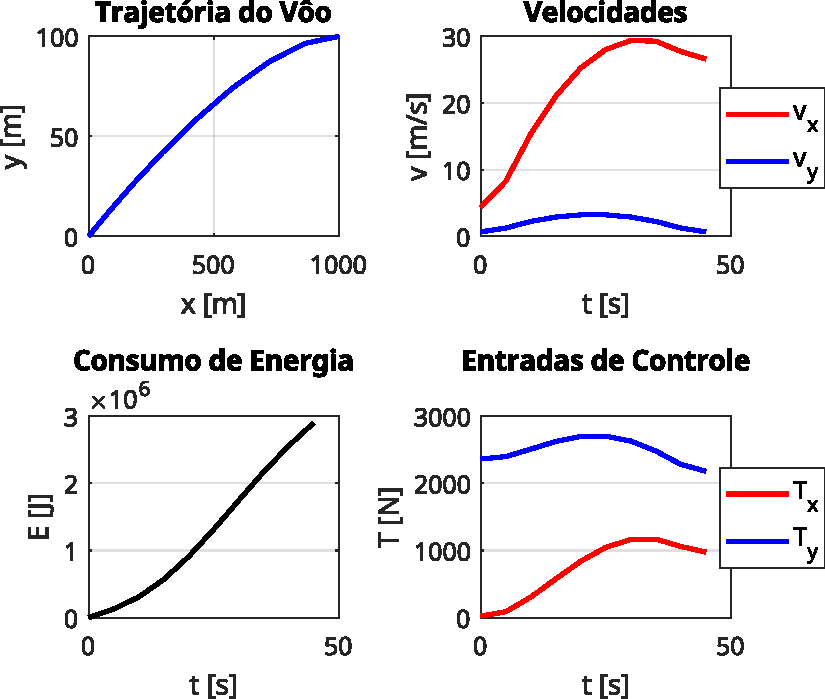
\includegraphics[width=0.75\textwidth]{Cap4/figuras/evtol-chute.pdf}
    \caption{Chute inicial para o problema de trajetória do eVTOL.}
    \label{fig:resultados-evtol-chute}
\end{figure}

Como opções do solver, utilizou-se uma sequência de refinamento da malha, com $n=[10, 20, 40, 80]$ pontos de colocação. Além disso, assim como no problema da braquistócrona, foram utilizadas diversas outras opções de parâmetros para que o solver convergisse para a solução ótima, como o uso de um algoritmo de otimização mais robusto e uma tolerância para a verificação de restrições mais restritiva.

Apesar dos esforços, o solver não encontrou um ótimo local nem mesmo nas iterações com menos pontos na malha. O melhor resultado obtido é apresentado na Figura \ref{fig:resultados-evtol}.

\begin{figure}[H]
    \centering
    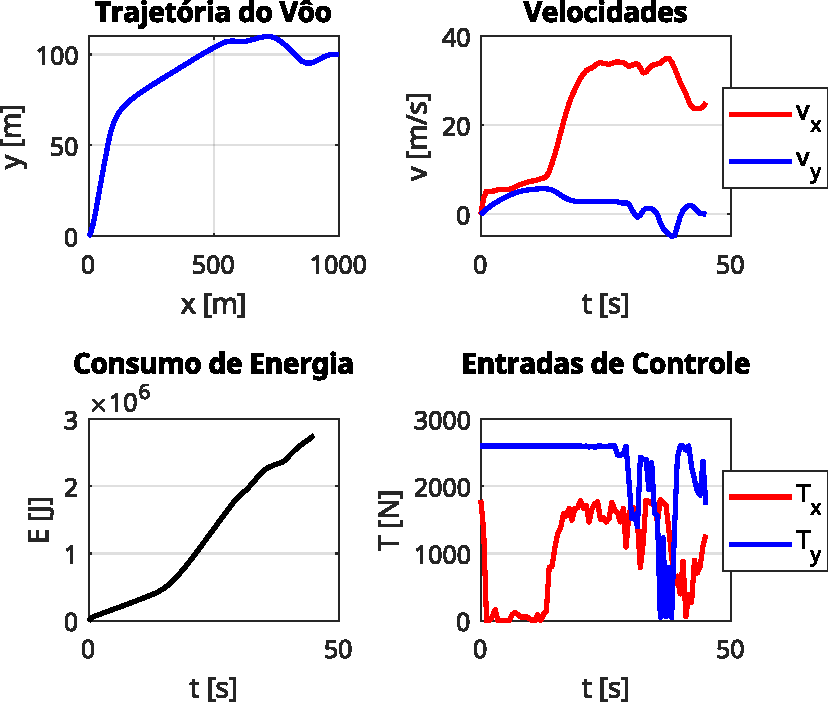
\includegraphics[width=0.75\textwidth]{Cap4/figuras/evtol.pdf}
    \caption{Trajetória ótima do problema de trajetória do eVTOL.}
    \label{fig:resultados-evtol}
\end{figure}

Apesar da solução não ser a ótima e as entradas de controle não serem suaves, a trajetória encontrada é fisicamente plausível e o consumo de energia é menor do que o da solução de referência, sendo $E=2,75484 \, \si{\mega\joule}$ para a solução obtida comparado a $E=2,94342 \, \si{\mega\joule}$ da referência. A Figura \ref{fig:resultados-evtol-comparacao} mostra a comparação entre a solução obtida e a solução de referência.

\begin{figure}[H]
    \centering
    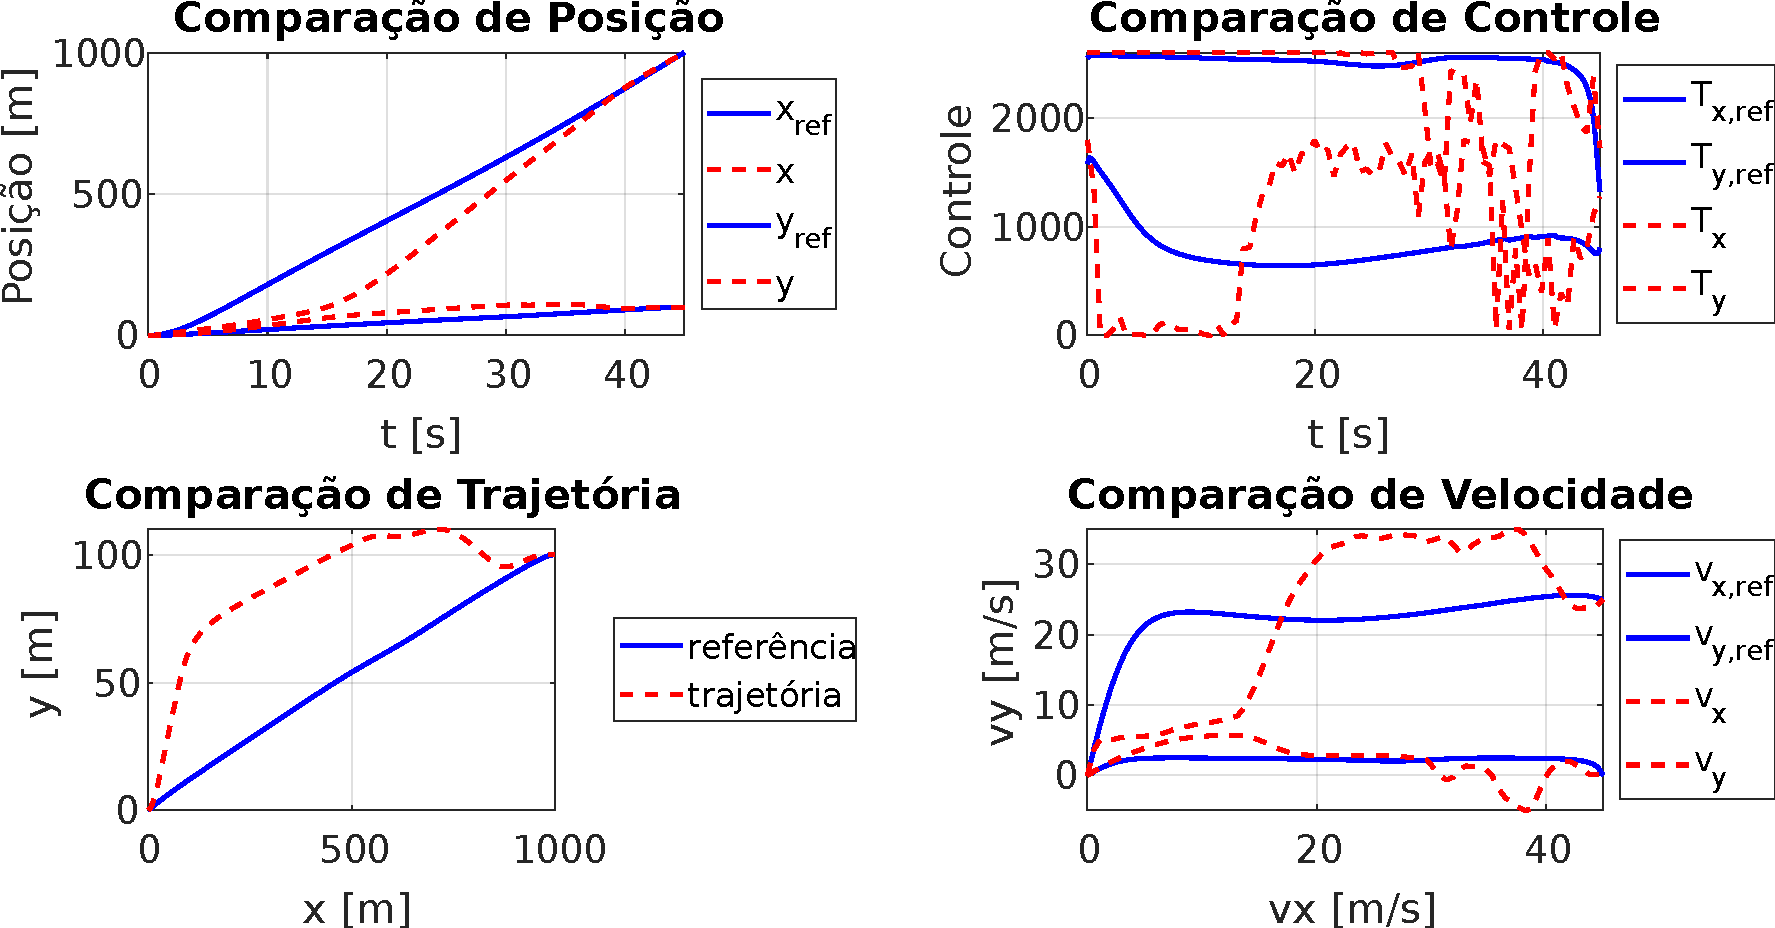
\includegraphics[width=\textwidth]{Cap4/figuras/evtol-comparacao.pdf}
    \caption{Comparação entre a solução obtida e a solução de referência.}
    \label{fig:resultados-evtol-comparacao}
\end{figure}

\begin{figure}[H]
    \centering
    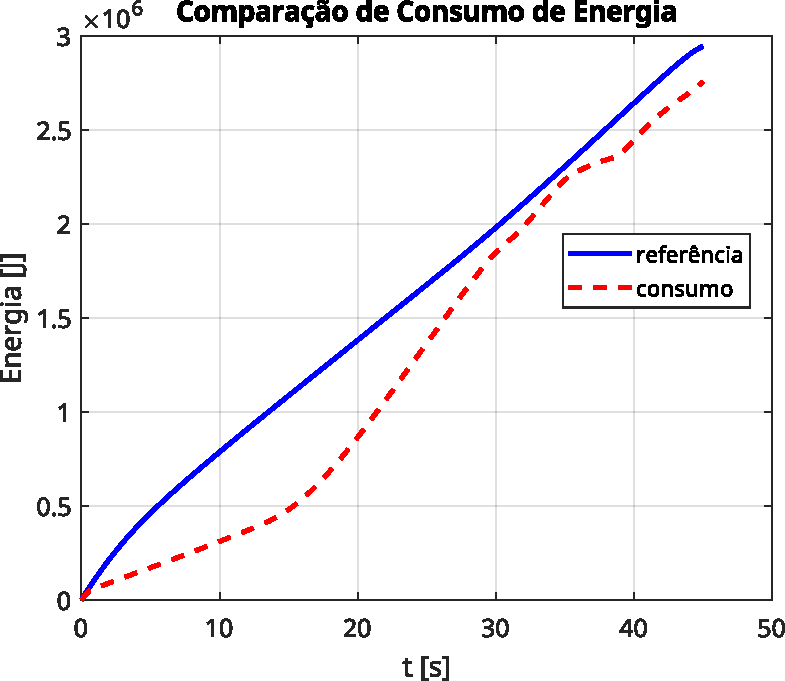
\includegraphics[width=0.65\textwidth]{Cap4/figuras/evtol-comparacao-energia.pdf}
    \caption{Comparação da energia.}
    \label{fig:resultados-evtol-comparacao-energia}
\end{figure}
